\chapter{Resultados e Análise}
\label{cap:resultados_analise}

Este capítulo apresenta os resultados obtidos a partir da aplicação das técnicas SHAP e LIME sobre o modelo de \textit{Rating} da Dívida Ativa da SEFAZ-DF. Em razão das restrições de sigilo e da remoção dos dados reais da versão final do projeto, todas as análises aqui reportadas foram conduzidas sobre bases sintéticas geradas pela estratégia \textit{GaussianCopula+log}, preservando-se a lógica de pré-processamento, o \textit{ensemble} de produção e as regras de pós-processamento descritas no Capítulo \ref{cap:metodologia}. O foco desta seção recai sobre três eixos: a importância global das variáveis no modelo, a concordância entre SHAP e LIME e a estabilidade das explicações locais produzidas pelo LIME.

\section{Panorama da Execução Experimental}

Os resultados consolidados abrangem os cinco \textit{setups} tributários considerados no projeto: \textit{ICMS}, \textit{ISS}, \textit{IPVA}, \textit{IPTU} e \textit{Taxas}. Em todos eles, a camada explicativa foi aplicada sobre o mesmo \textit{ensemble} de produção, composto por três modelos XGBoost por imposto, com agregação por média das probabilidades e posterior normalização conforme os parâmetros operacionais do \textit{Rating}. Essa escolha metodológica permitiu avaliar a explicabilidade sem alterar o mecanismo decisório efetivamente utilizado no sistema original.

Entre os cinco \textit{setups}, o caso do \textit{ICMS} concentrou o conjunto mais completo de artefatos visuais e tabulares, incluindo \textit{summary plots}, \textit{waterfall plots}, \textit{decision plots}, explicações locais em LIME e métricas de estabilidade. Por essa razão, ele é utilizado neste capítulo como estudo de caso principal, enquanto os demais impostos cumprem o papel de validação comparativa transversal.

No caso do \textit{ICMS}, a execução do notebook principal sobre 50.000 amostras sintéticas resultou em 6.392 ocorrências classificadas como A, 10.822 como B, 31.433 como C e 1.353 como D. Das CDAs de \textit{rating} A, 5.245 receberam essa classe pela regra de sobreposição associada à situação da CDA (parcelamento ou suspensão), e apenas 1.147, cerca de 2,3\% da amostra, chegaram a ela pela probabilidade estimada pelo modelo. Isso mostra que a análise explicativa precisa considerar não apenas o modelo, mas também a lógica complementar de negócio presente no processo decisório, e evidencia o desbalanceamento entre classes discutido na Seção \ref{subsec:desbalanceamento}.

\section{Importância Global das Variáveis no \textit{Ensemble} de Produção}

A análise global com SHAP, detalhada para o \textit{ICMS}, mostrou que a decisão do \textit{ensemble} é fortemente influenciada por um núcleo relativamente pequeno de variáveis. A Figura \ref{fig:shap_global_icms} apresenta a importância média global das variáveis nesse \textit{setup}, evidenciando a predominância de fatores relacionados ao histórico de regularização, ao volume agregado de dívidas e ao tempo sem movimentação da dívida.

\begin{figure}[H]
    \centering
    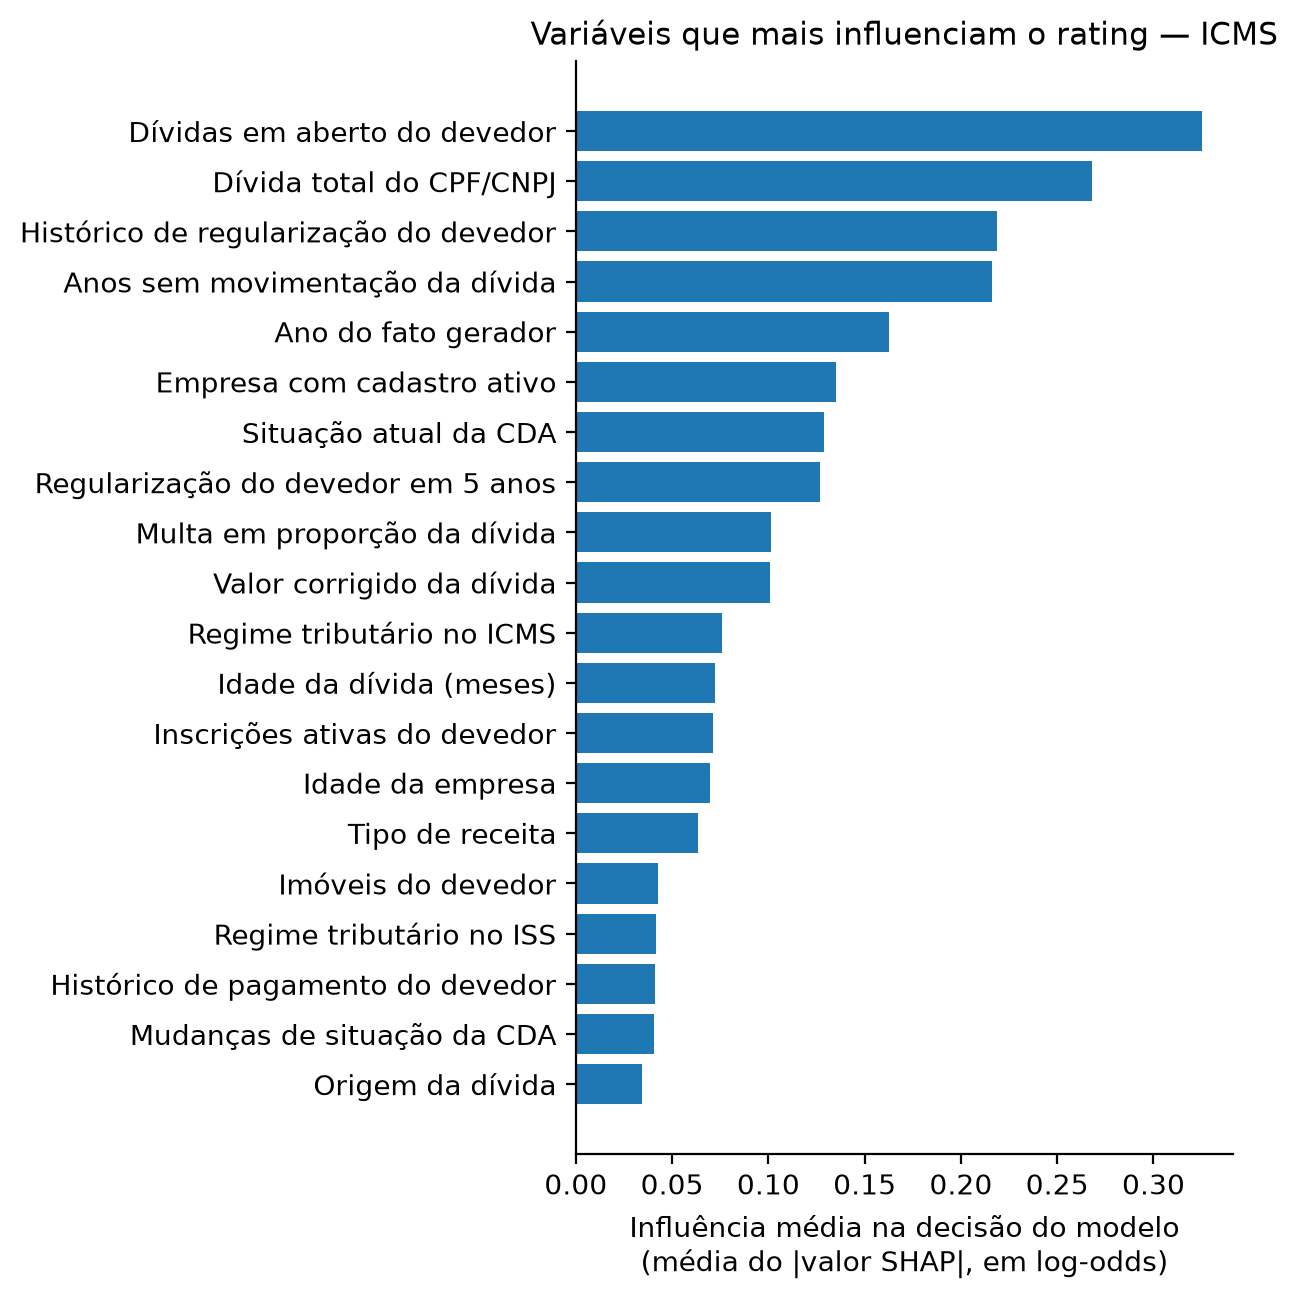
\includegraphics[width=0.92\textwidth]{figuras/xai/shap_summary_bar_icms.png}
    \caption[Importância global das variáveis segundo o SHAP no ICMS]{Importância global das 20 variáveis mais relevantes para o \textit{ensemble} de produção do ICMS, calculada sobre 50.000 CDAs sintéticas. Cada barra é a média, sobre todas as CDAs, do valor absoluto da contribuição SHAP da variável, já combinada entre os três modelos XGBoost; o eixo horizontal está na escala interna do modelo (logaritmo da razão de chances de pagamento). Quanto maior a barra, mais a variável altera, em média, a probabilidade estimada, para mais ou para menos; o gráfico não indica o sentido do efeito. As quatro primeiras variáveis, que tratam da quantidade de dívidas abertas no núcleo do contribuinte, do valor total devido pelo CPF ou CNPJ, do histórico de regularização e dos anos sem movimentação da dívida, respondem sozinhas por 43\% da importância total das 24 variáveis do modelo.}
    \label{fig:shap_global_icms}

\end{figure}

A Tabela \ref{tab:icms_ensemble_importance} resume as dez variáveis de maior relevância média no \textit{ensemble} de \textit{ICMS}. Além da média dos valores absolutos de SHAP, apresenta-se o desvio padrão e o coeficiente de variação entre os três modelos do conjunto, permitindo avaliar a consistência interna do \textit{ensemble}.

\begin{table}[H]
    \centering
    \caption[Dez variáveis mais importantes do \textit{ensemble} do ICMS e sua variação entre os três modelos]{Dez variáveis mais importantes do \textit{ensemble} do ICMS e sua variação entre os três modelos XGBoost que o compõem, calculadas sobre 50.000 CDAs sintéticas. A média SHAP é a média, entre os três modelos, da importância global de cada um (média do valor absoluto de SHAP). O desvio padrão e o coeficiente de variação (desvio dividido pela média) medem quanto os três modelos discordam sobre essa importância: valores próximos de zero indicam que os modelos atribuem à variável praticamente o mesmo peso. Apenas a multa em proporção da dívida supera 0,15 de coeficiente de variação, o que indica um \textit{ensemble} internamente coerente.}
    \label{tab:icms_ensemble_importance}
    \small
    \renewcommand{\arraystretch}{1.2}
    \begin{tabularx}{\textwidth}{>{\raggedright\arraybackslash}p{6.2cm}CCC}
        \toprule
        \textbf{Variável} & \textbf{Média SHAP} & \textbf{Desvio padrão} & \textbf{Coeficiente de variação} \\
        \midrule
        Dívidas em aberto do devedor            & 0,3250 & 0,0146 & 0,0451 \\
        Dívida total do CPF/CNPJ                & 0,2682 & 0,0083 & 0,0309 \\
        Histórico de regularização do devedor   & 0,2188 & 0,0102 & 0,0467 \\
        Anos sem movimentação da dívida         & 0,2161 & 0,0025 & 0,0114 \\
        Ano do fato gerador                     & 0,1625 & 0,0151 & 0,0928 \\
        Empresa com cadastro ativo              & 0,1352 & 0,0096 & 0,0710 \\
        Situação atual da CDA                   & 0,1289 & 0,0067 & 0,0520 \\
        Regularização do devedor em 5 anos      & 0,1267 & 0,0035 & 0,0277 \\
        Multa em proporção da dívida            & 0,1016 & 0,0390 & 0,3838 \\
        Valor corrigido da dívida               & 0,1006 & 0,0147 & 0,1457 \\
        \bottomrule
    \end{tabularx}
\end{table}

Os resultados da Tabela \ref{tab:icms_ensemble_importance} indicam que o \textit{ensemble} não é composto por modelos semanticamente contraditórios. Entre os dez fatores mais relevantes de cada modelo individual, nove aparecem simultaneamente nos três membros do conjunto, ao passo que a união total dos \textit{top-10} contém apenas onze variáveis distintas. Em termos práticos, isso significa que a média dos valores de SHAP entre os modelos preserva uma estrutura explicativa coerente, reforçando a adequação dessa estratégia para representar a decisão agregada do \textit{ensemble}.

Também é relevante observar a natureza substantiva das variáveis mais importantes. Em vez de sinais periféricos, predominam atributos diretamente associados à recuperabilidade do crédito, tais como a quantidade de dívidas abertas no núcleo do contribuinte, o valor total de dívida associado ao CPF ou CNPJ, o histórico de regularização e o tempo sem movimentação da dívida. Isso fortalece a interpretação de que o modelo organiza sua decisão a partir de critérios materialmente plausíveis no contexto da cobrança tributária.

\section{Comparação entre SHAP e LIME}

Para avaliar a utilidade comparativa das duas técnicas de explicabilidade, foram analisadas explicações locais representativas de cada \textit{setup} e de cada classe de \textit{rating}. A Tabela \ref{tab:comparacao_setups} apresenta as médias, por imposto, da concordância entre os \textit{top-5} fatores de SHAP e LIME, medida por \textit{Jaccard@5} e \textit{Rank-Biased Overlap} (RBO@5), bem como da estabilidade interna do LIME ao longo de múltiplas execuções.

\begin{table}[H]
    \centering
    \caption[Concordância entre SHAP e LIME e estabilidade do LIME, por \textit{setup}]{Concordância entre SHAP e LIME e estabilidade do LIME, por \textit{setup}. Cada valor é a média dos quatro casos representativos do \textit{setup} (uma CDA sintética por classe de \textit{rating}). \textit{Jaccard}@5 é a fração de variáveis em comum entre as cinco principais de cada método (0 a 1). RBO@5 mede a mesma concordância dando mais peso às primeiras posições; na forma truncada utilizada, seu valor máximo é 0,41, e não 1. A estabilidade do LIME é o \textit{Jaccard}@5 médio entre 30 execuções do LIME com sementes diferentes (1 indica explicações idênticas). A última coluna é o número médio de variáveis distintas que apareceram entre as cinco principais ao longo dessas 30 execuções; quanto menor, mais estável. Em todas as colunas, exceto a última, valores maiores indicam mais concordância ou estabilidade.}
    \label{tab:comparacao_setups}
    \small
    \renewcommand{\arraystretch}{1.2}
    \begin{tabularx}{\textwidth}{LCCCC}
        \toprule
        \textbf{\textit{Setup}} & \textbf{Jaccard@5} & \textbf{RBO@5} & \textbf{Estabilidade do LIME} & \textbf{Variáveis distintas no \textit{top-5}} \\
        \midrule
        ICMS  & 0,3492 & 0,1142 & 0,6920 & 11,25 \\
        ISS   & 0,5030 & 0,2375 & 0,8438 & 8,25 \\
        IPVA  & 0,3046 & 0,1697 & 0,7636 & 9,25 \\
        IPTU  & 0,4435 & 0,2589 & 0,8973 & 6,50 \\
        Taxas & 0,3393 & 0,1980 & 0,7970 & 8,75 \\
        \bottomrule
    \end{tabularx}
\end{table}

Os resultados da Tabela \ref{tab:comparacao_setups} mostram que a concordância entre SHAP e LIME é parcial, e não total, em todos os cenários observados. Como o RBO@5 truncado tem teto de 0,41 (Seção \ref{sec:procedimentos_xai}), as médias entre 0,11 e 0,26 correspondem a algo entre 28\% e 63\% da concordância máxima possível nas primeiras posições. O \textit{setup} com maior alinhamento médio foi o \textit{ISS}, com \textit{Jaccard@5} de 0,5030, seguido por \textit{IPTU}. Na extremidade oposta, \textit{IPVA} apresentou a menor concordância média, com 0,3046. O caso de \textit{ICMS} merece atenção especial: embora seja o \textit{setup} mais rico em artefatos e o principal estudo de caso do trabalho, ele não foi o mais alinhado entre os métodos, o que o torna particularmente útil para discutir as tensões metodológicas entre explicabilidade baseada em teoria dos jogos e explicabilidade local por aproximação.

A análise por classe de \textit{rating}, sintetizada na Tabela \ref{tab:comparacao_ratings}, revela um segundo padrão importante: os grupos mais extremos tendem a apresentar maior concordância entre SHAP e LIME do que os grupos intermediários.

\begin{table}[H]
    \centering
    \caption[Concordância entre SHAP e LIME e estabilidade do LIME, por classe de \textit{rating}]{Concordância entre SHAP e LIME e estabilidade do LIME, por classe de \textit{rating}. Cada valor é a média dos cinco casos da classe (uma CDA sintética representativa por imposto). As métricas são as mesmas da Tabela \ref{tab:comparacao_setups}: \textit{Jaccard}@5 varia de 0 a 1, RBO@5 tem teto de 0,41, a estabilidade do LIME é a concordância média entre 30 execuções, e a última coluna conta as variáveis distintas que passaram pelo \textit{top-5} do LIME nessas execuções. As classes extremas (A e D) apresentam o LIME mais estável, e a classe D, a maior concordância entre os métodos.}
    \label{tab:comparacao_ratings}
    \small
    \renewcommand{\arraystretch}{1.2}
    \begin{tabularx}{\textwidth}{LCCCC}
        \toprule
        \textbf{\textit{Rating}} & \textbf{Jaccard@5} & \textbf{RBO@5} & \textbf{Estabilidade do LIME} & \textbf{Variáveis distintas no \textit{top-5}} \\
        \midrule
        A & 0,3294 & 0,1708 & 0,8104 & 8,60 \\
        B & 0,4405 & 0,1951 & 0,7618 & 9,00 \\
        C & 0,2937 & 0,1882 & 0,7632 & 9,80 \\
        D & 0,4881 & 0,2286 & 0,8596 & 7,80 \\
        \bottomrule
    \end{tabularx}
\end{table}

Na Tabela \ref{tab:comparacao_ratings}, o \textit{rating} D apresenta a maior média de concordância entre os métodos, enquanto o \textit{rating} C exibe a menor. Esse comportamento sugere que, em situações mais extremas, os fatores decisórios do modelo tornam-se mais nítidos e, por consequência, mais facilmente capturados por técnicas explicativas distintas. Já nos casos intermediários, a decisão parece depender de interações mais sensíveis ao método de interpretação empregado.

Os casos individuais corroboram essa leitura. As melhores concordâncias observadas ocorreram em \textit{ISS-D} e \textit{IPTU-D}, ambos com \textit{Jaccard@5} de 0,6667 e \textit{RBO@5} de 0,3062, o equivalente a 75\% do teto da métrica. Em contraste, o caso de \textit{ICMS-A} foi o mais divergente da base, com \textit{Jaccard@5} de 0,1111 e \textit{RBO@5} de 0,1033. Esse resultado é metodologicamente relevante porque demonstra que a escolha da técnica explicativa não é indiferente: em determinados cenários, a interpretação da mesma decisão algorítmica pode variar de maneira substantiva conforme o método utilizado.

Apesar dessa divergência parcial, um núcleo explicativo recorrente foi identificado entre SHAP e LIME. Considerando os vinte casos analisados no conjunto dos cinco \textit{setups}, as variáveis que mais frequentemente apareceram simultaneamente no \textit{top-5} dos dois métodos foram as dívidas em aberto do devedor, o histórico de regularização do devedor, os anos sem movimentação da dívida, a dívida total do CPF/CNPJ e a idade da dívida (Tabela \ref{tab:glossario_variaveis}). Em outras palavras, ainda que os métodos discordem na ordenação fina e na composição completa das explicações locais, ambos convergem em torno de um conjunto estruturante de fatores ligados à exposição do contribuinte, ao seu histórico de regularização e à antiguidade ou persistência da dívida.

\section{Estabilidade das Explicações Locais com LIME}

Além da comparação direta com SHAP, a estabilidade do LIME foi examinada em trinta execuções por caso, variando-se a semente aleatória. A análise mostrou que o LIME não se comporta de forma caótica, mas tampouco apresenta estabilidade uniforme em todos os contextos. A Figura \ref{fig:lime_heatmap_icms_d} ilustra a estabilidade do \textit{top-5} do LIME para o \textit{rating} D no \textit{setup} de \textit{ICMS}, destacando as variáveis que se repetem ao longo das execuções.

\begin{figure}[H]
    \centering
    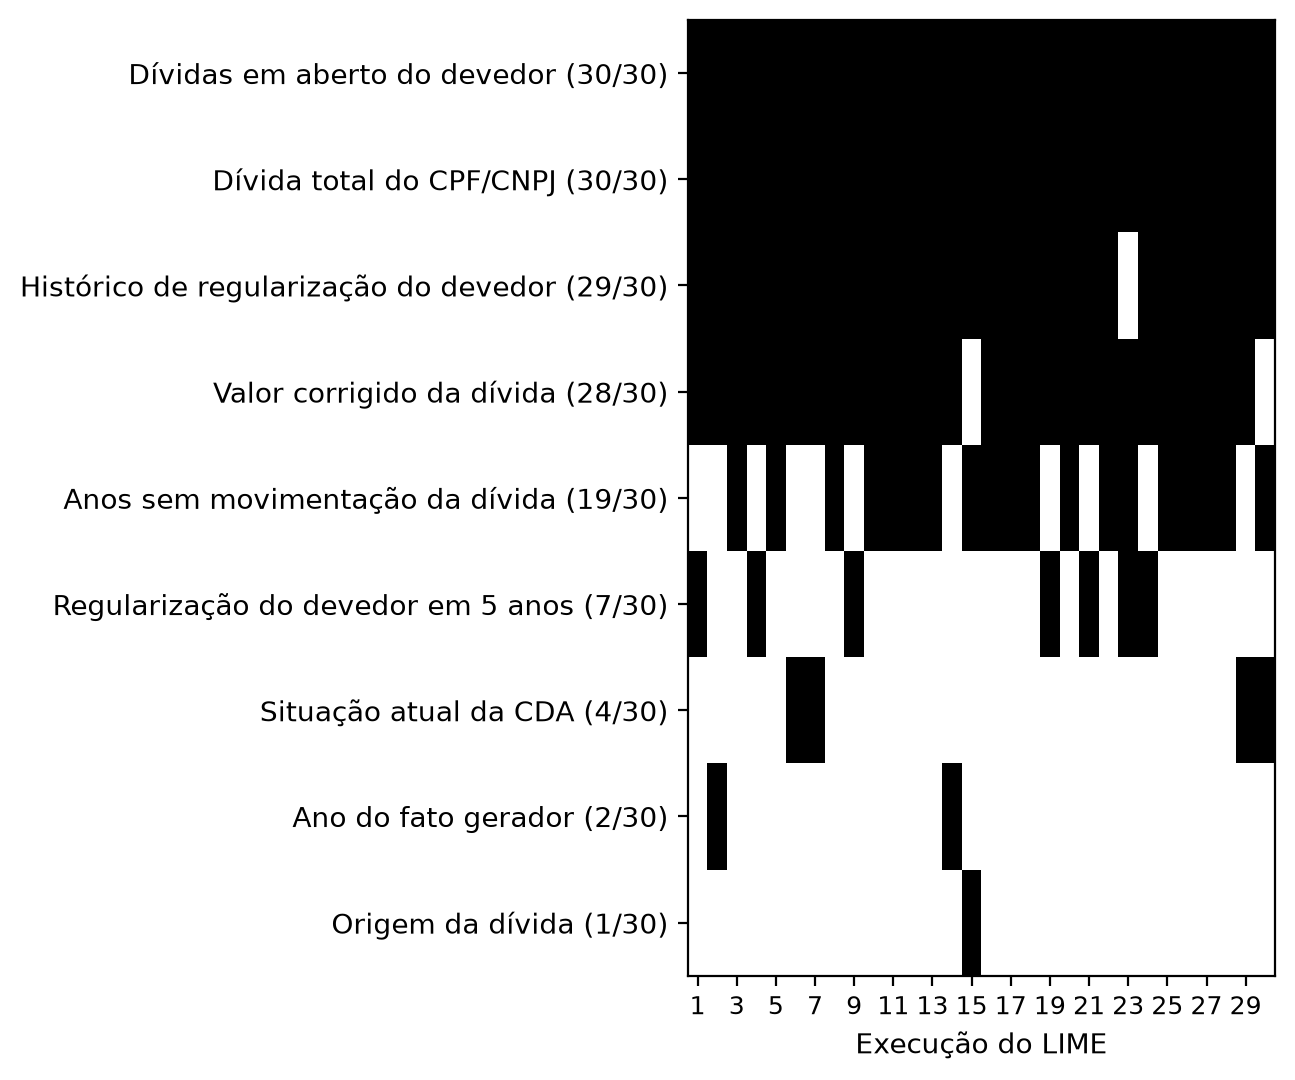
\includegraphics[width=\textwidth]{figuras/xai/lime_stability_heatmap_rating_D_icms.png}
    \caption[Estabilidade do \textit{top-5} do LIME em 30 execuções para uma CDA de \textit{rating} D no ICMS]{Estabilidade das explicações do LIME para uma mesma CDA sintética de \textit{rating} D no ICMS, explicada 30 vezes com sementes aleatórias de 42 a 71 (eixo horizontal). Cada linha é uma variável, e uma célula preta indica que, naquela execução, a variável ficou entre as cinco mais importantes; o número entre parênteses informa em quantas das 30 execuções isso ocorreu. Linhas totalmente pretas são fatores que o LIME identifica sempre; linhas intermitentes revelam fatores que entram e saem da explicação apenas por efeito da amostragem aleatória. Neste caso, quatro variáveis aparecem em pelo menos 28 das 30 execuções, enquanto a quinta posição alterna entre outras cinco.}
    \label{fig:lime_heatmap_icms_d}

\end{figure}

Em termos agregados, os melhores resultados de estabilidade ocorreram em \textit{ISS-D} e \textit{IPTU-D}, ambos com \textit{jaccard\_pair\_mean} de 0,9778, seguidos por \textit{IPTU-C} (0,9364) e \textit{ISS-A} (0,9351). Na outra extremidade, os menores valores apareceram em \textit{ISS-C} (0,6229), \textit{ICMS-A} (0,6597), \textit{ICMS-C} (0,6635) e \textit{ICMS-B} (0,6860). Esses resultados indicam que o LIME pode ser bastante estável em alguns cenários, mas essa estabilidade depende do contexto analítico e da observação selecionada.

Outro aspecto importante foi a recorrência da principal variável de cada explicação. Em todos os casos analisados, a variável mais frequente do \textit{top-5} do LIME apareceu em 100\% das execuções. No entanto, a quantidade de variáveis distintas presentes no \textit{top-5} ao longo das trinta repetições variou substancialmente. Em \textit{ICMS-A}, por exemplo, treze variáveis diferentes apareceram no \textit{top-5}, ao passo que em \textit{ISS-D} e \textit{IPTU-D} esse número foi de apenas seis. Isso significa que o primeiro fator local identificado pelo LIME tende a ser robusto, mas os fatores subsequentes podem rotacionar de forma mais sensível à perturbação dos dados.

Do ponto de vista da auditoria fiscal, essa característica tem implicações diretas. O LIME mostra-se útil como mecanismo de inspeção local e como ferramenta de comunicação para partes interessadas não técnicas, especialmente quando se busca uma explicação textual ou visual rápida. Contudo, sua variabilidade nas posições inferiores do \textit{ranking} recomenda cautela quando se pretende utilizá-lo como fundamento principal de motivação administrativa.

\section{Estudo de Caso Local: \textit{Rating} D em ICMS}

No estudo de caso principal, o notebook do \textit{framework} do auditor foi executado sobre uma CDA sintética classificada como \textit{rating} D no \textit{setup} de \textit{ICMS}. A Figura \ref{fig:waterfall_icms_d} apresenta o respectivo \textit{waterfall plot}, no qual se observa a decomposição local da predição em fatores que favorecem e fatores que dificultam a regularização.

\begin{figure}[H]
    \centering
    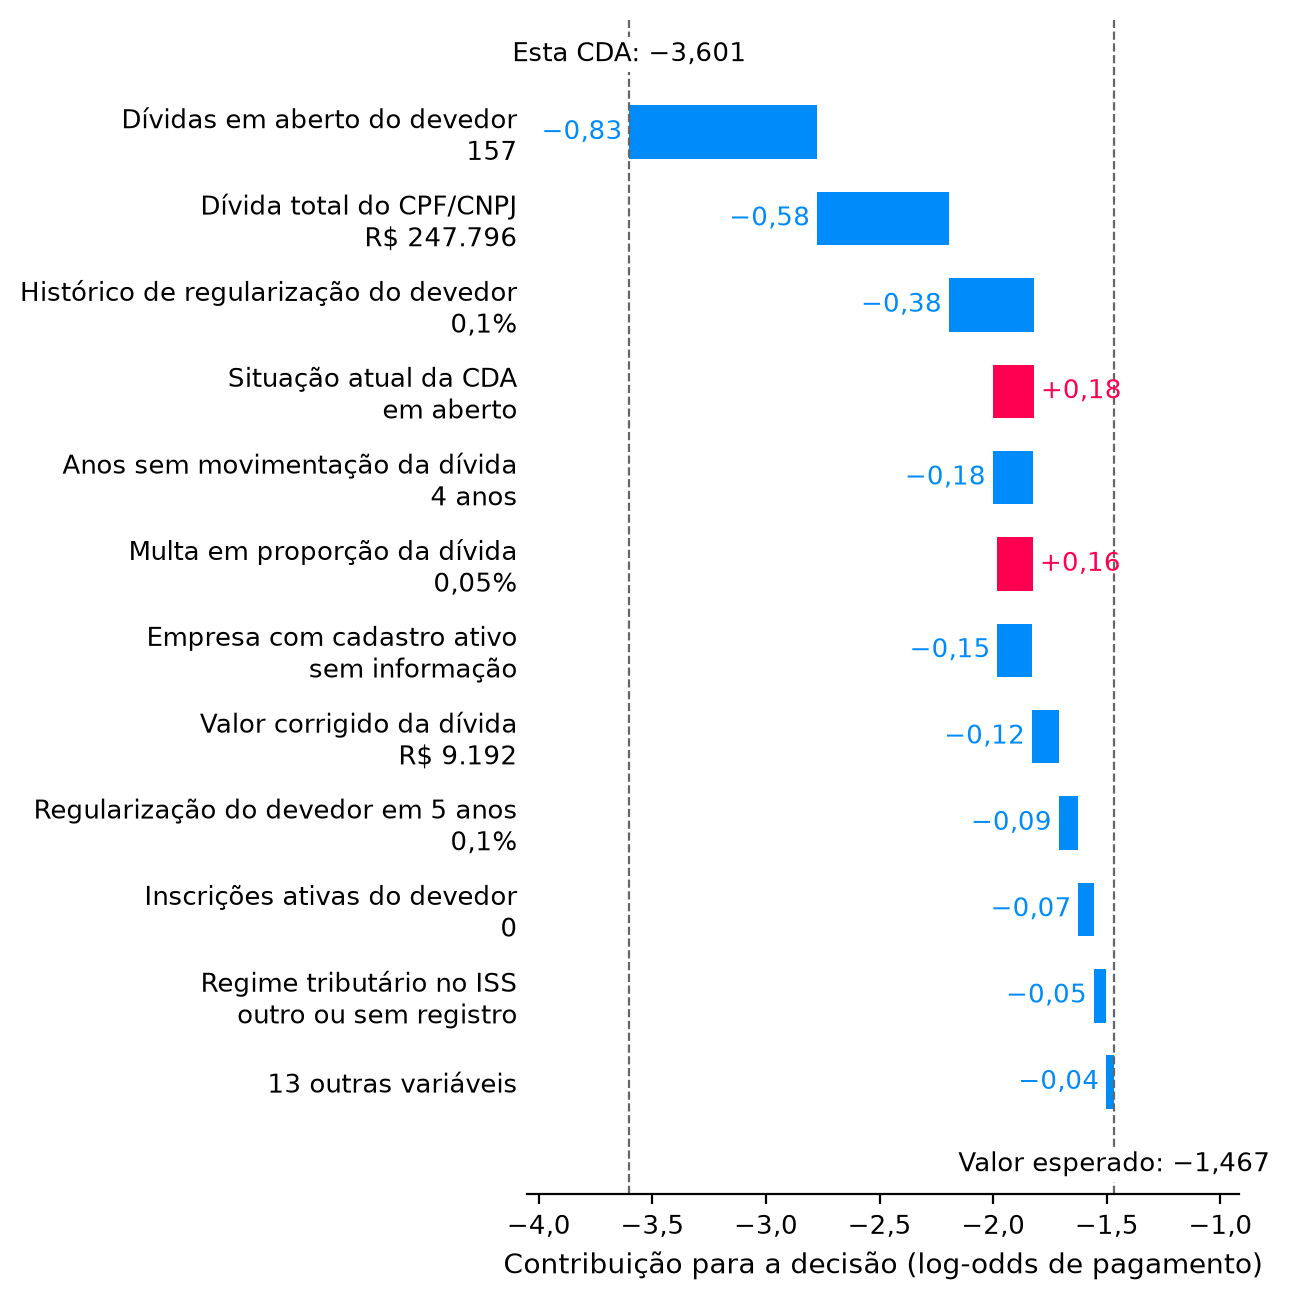
\includegraphics[width=\textwidth]{figuras/xai/shap_waterfall_rating_D_icms.png}
    \caption[Explicação SHAP de uma CDA sintética de \textit{rating} D no ICMS]{Explicação SHAP (gráfico de cascata) de uma CDA sintética de \textit{rating} D no ICMS, escolhida por ter a probabilidade mais próxima da mediana da classe. A leitura começa na base do gráfico, na linha tracejada do valor esperado do modelo ($-1{,}467$), que corresponde à CDA média, e sobe barra a barra. Cada barra é a contribuição de uma variável, cujo valor nesta CDA aparece abaixo do nome: barras azuis reduzem a chance de pagamento, e barras vermelhas a aumentam. A linha tracejada do topo ($-3{,}601$) é a saída final do modelo para esta CDA, equivalente a uma probabilidade normalizada de 0,022, abaixo do limite de 0,03 da classe D. Os valores estão na escala interna do modelo (logaritmo da razão de chances). As três maiores contribuições negativas vêm do grande número de dívidas em aberto do devedor (157), do alto valor total devido pelo CPF ou CNPJ e da ausência de histórico de regularização.}
    \label{fig:waterfall_icms_d}

\end{figure}

No caso analisado, destacaram-se como fatores de maior peso negativo a quantidade de dívidas abertas no núcleo do contribuinte, o valor total da dívida associada ao CPF ou CNPJ e o histórico de regularização total, seguidos, com peso menor, pelos anos sem movimentação da dívida. Em sentido oposto, a situação inicial da CDA e o valor da multa contribuíram positivamente, mas sem força suficiente para deslocar a probabilidade final para uma classe de maior recuperabilidade. Esse tipo de visualização é particularmente relevante para o objetivo do trabalho, pois traduz a saída numérica do modelo em uma narrativa causal localmente interpretável, aproximando o resultado algorítmico da lógica de fundamentação exigida em processos administrativos.

\section{Efeito do Desbalanceamento Micro}
\label{sec:resultado_desbalanceamento}

A Figura \ref{fig:desbalanceamento} e a Tabela \ref{tab:desbalanceamento} apresentam o resultado do experimento descrito na Seção \ref{sec:experimento_desbalanceamento}. As duas variantes produziram comportamentos opostos.

\begin{figure}[H]
    \centering
    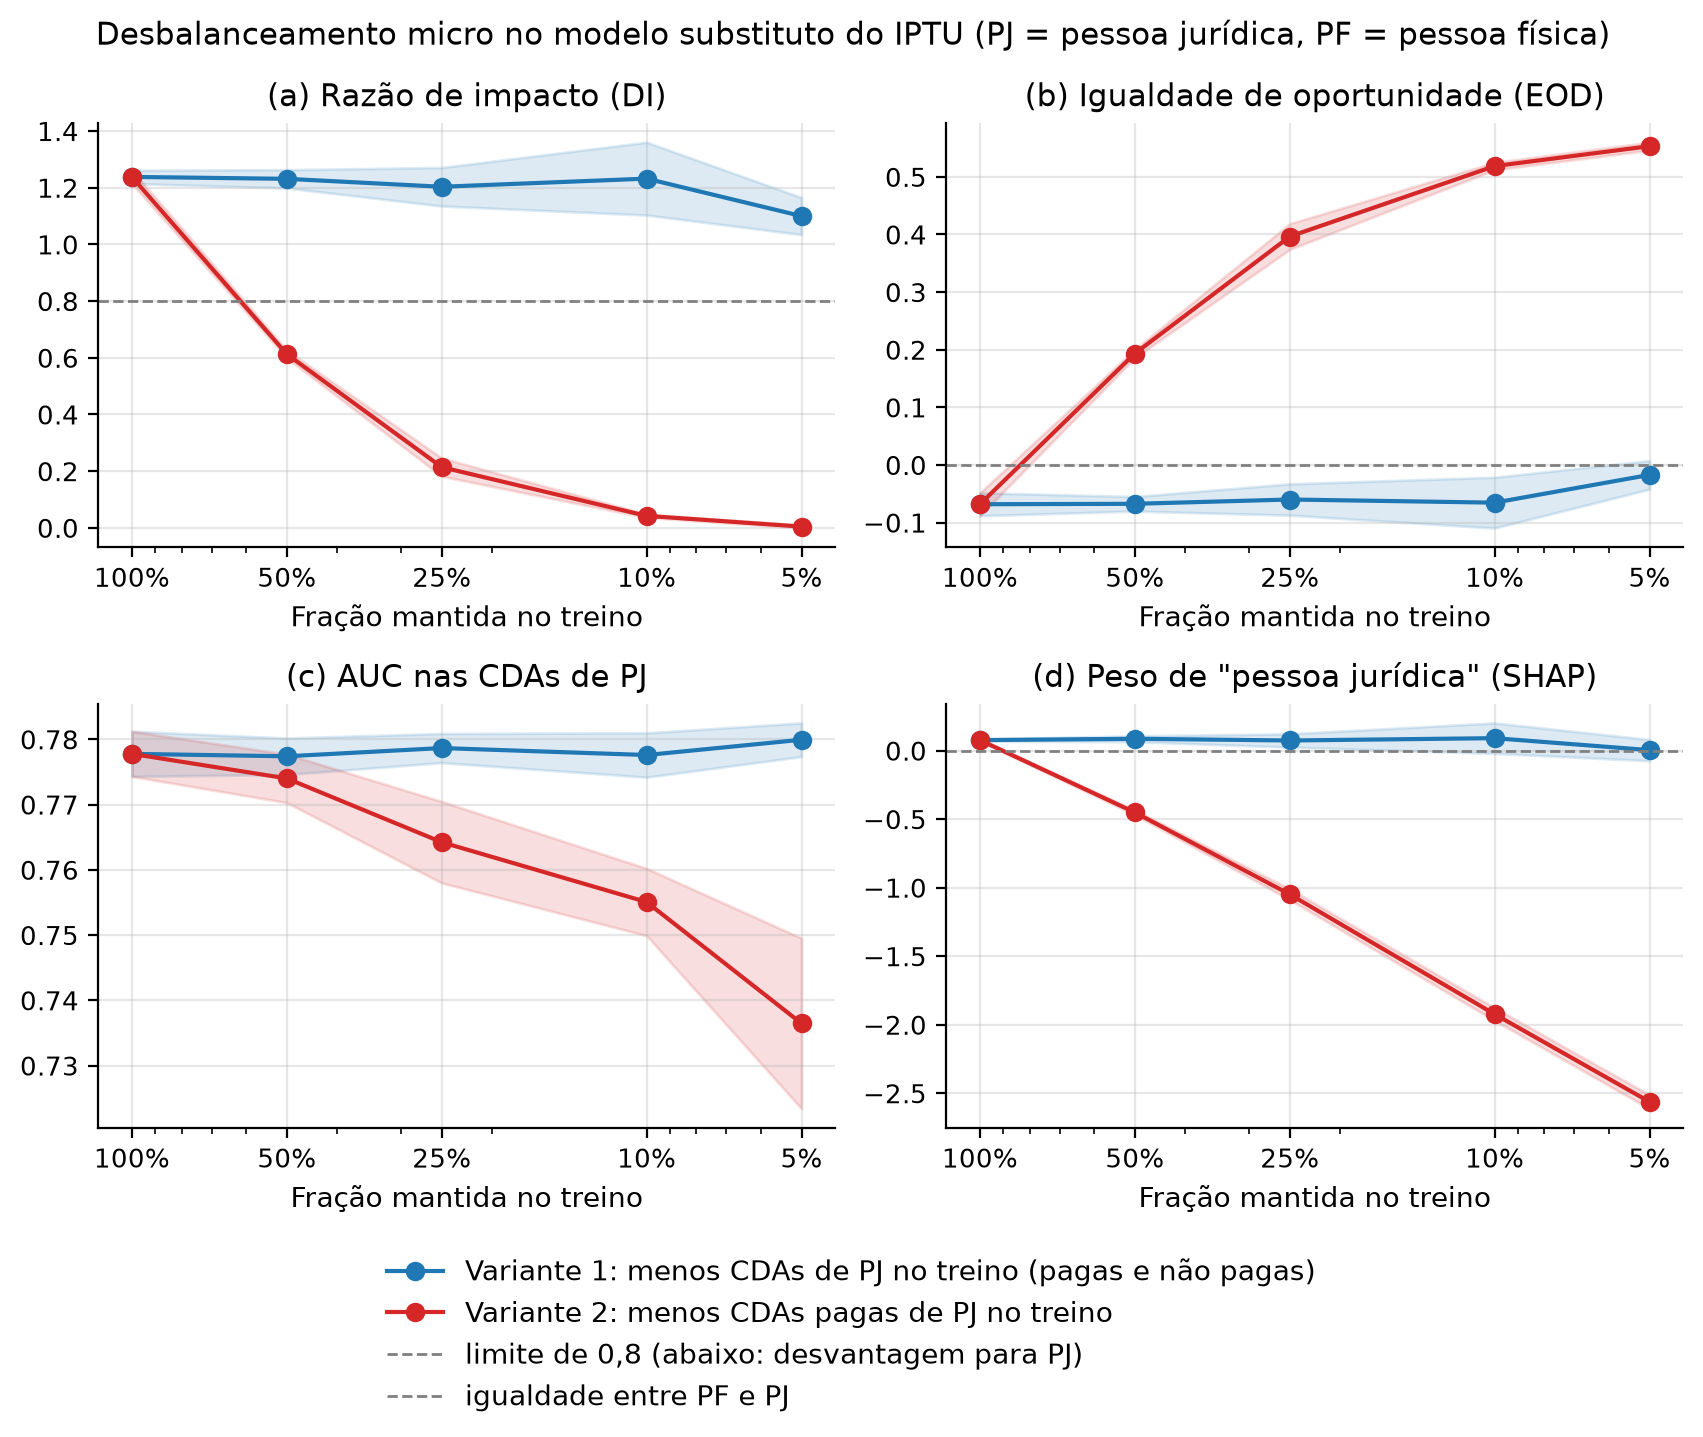
\includegraphics[width=\textwidth]{figuras/xai/desbalanceamento_iptu_se_cnpj.png}
    \caption[Efeito do desbalanceamento micro sobre o modelo substituto do IPTU]{Efeito do desbalanceamento micro sobre um modelo XGBoost substituto, treinado com as CDAs sintéticas do IPTU, comparando contribuintes pessoa jurídica (PJ) e pessoa física (PF). O eixo horizontal de cada painel é a fração das CDAs de PJ mantida no treino, decrescente da esquerda para a direita (de 100\%, sem manipulação, até 5\%). A linha azul remove CDAs de PJ em geral (variante 1); a linha vermelha remove apenas as CDAs de PJ que foram pagas (variante 2). Cada ponto é a média de cinco treinamentos, e a faixa sombreada é um desvio padrão. Os painéis mostram, no conjunto de teste inalterado: (a) a razão de impacto (DI), isto é, a porcentagem de CDAs de PJ com \textit{rating} A ou B dividida pela de PF, em que valores abaixo da linha de 0,8 indicam impacto desproporcional contra PJ; (b) a diferença de igualdade de oportunidade (EOD), isto é, a porcentagem dos bons pagadores PF classificados como A ou B menos a dos bons pagadores PJ, em que valores acima de zero indicam que bons pagadores PJ são reconhecidos com menos frequência; (c) a AUC nas CDAs de PJ; e (d) a contribuição SHAP média da variável ``pessoa jurídica'' para as CDAs de PJ, em que valores negativos indicam que o modelo passou a penalizar o próprio fato de o contribuinte ser PJ. Apenas a variante 2 produz viés.}
    \label{fig:desbalanceamento}

\end{figure}

Reduzir o tamanho do grupo PJ (variante 1) praticamente não alterou o modelo. Mesmo com apenas 5\% das CDAs de PJ no treino, cerca de 42 delas pagas, a AUC no grupo permaneceu em 0,78 e a razão de impacto variou de 1,24 para 1,10, ainda favorável a PJ. Nos dados sintéticos, a relação entre as características da CDA e o pagamento é semelhante para PF e PJ, de modo que o modelo aprende com as CDAs de PF o que precisa para classificar as de PJ. A sub-representação de um grupo, isoladamente, não gerou viés.

Reduzir apenas os pagadores PJ (variante 2) teve efeito imediato. Com metade das CDAs pagas de PJ, a razão de impacto caiu de 1,24 para 0,61, abaixo do limite de 0,8, e a diferença de igualdade de oportunidade passou de $-0{,}07$ para $+0{,}19$: entre os contribuintes PJ que de fato pagaram, a proporção classificada como A ou B caiu de 62,5\% para 36,4\%, enquanto a de PF se manteve em 55,7\%. Com 5\% dos pagadores, praticamente nenhuma CDA de PJ recebeu classificação favorável. Vale notar que, no cenário de 5\%, a variante 2 manteve no treino cerca de 44 CDAs pagas de PJ, o mesmo número da variante 1 no mesmo nível. O que produziu o viés não foi a quantidade de exemplos, mas a proporção distorcida de pagadores dentro do grupo.

\begin{table}[H]
    \centering
    \caption[Métricas de performance e de viés do modelo substituto em cenários selecionados]{Métricas de performance e de viés do modelo substituto do IPTU em cenários selecionados, medidas no mesmo conjunto de teste (15.000 CDAs sintéticas com proporções naturais). Cada valor é a média de cinco treinamentos. ``PJ pagas'' é o número de CDAs de pessoa jurídica com pagamento que o modelo viu no treinamento. ``A ou B (PJ)'' é a fração de CDAs de PJ classificadas como A ou B (decisão favorável); a de PF ficou em 0,24 em todos os cenários. DI abaixo de 0,8 e EOD acima de zero indicam desvantagem para PJ. ``Peso PJ'' é a contribuição SHAP média, em log-odds, da variável ``pessoa jurídica'' nas CDAs de PJ; valores negativos indicam que o modelo penaliza o contribuinte por ser PJ.}
    \label{tab:desbalanceamento}
    \small
    \renewcommand{\arraystretch}{1.2}
    \begin{tabularx}{\textwidth}{>{\raggedright\arraybackslash}p{2.8cm}CCCCCCC}
        \toprule
        \textbf{Cenário} & \textbf{PJ pagas} & \textbf{AUC geral} & \textbf{AUC PJ} & \textbf{A ou B (PJ)} & \textbf{DI} & \textbf{EOD} & \textbf{Peso PJ} \\
        \midrule
        Sem alteração    & 888 & 0,782 & 0,778 & 0,303 & 1,24 & $-0{,}07$ & $+0{,}08$ \\
        Variante 1, 5\%  &  42 & 0,781 & 0,780 & 0,268 & 1,10 & $-0{,}02$ & $+0{,}00$ \\
        Variante 2, 50\% & 444 & 0,777 & 0,774 & 0,149 & 0,61 & $+0{,}19$ & $-0{,}45$ \\
        Variante 2, 25\% & 222 & 0,763 & 0,764 & 0,052 & 0,21 & $+0{,}40$ & $-1{,}05$ \\
        Variante 2, 5\%  &  44 & 0,726 & 0,736 & 0,001 & 0,00 & $+0{,}55$ & $-2{,}56$ \\
        \bottomrule
    \end{tabularx}
\end{table}

Dois resultados merecem destaque. O primeiro é que a performance agregada esconde o viés: no cenário de 50\%, a AUC geral passou de 0,782 para 0,777, uma variação que dificilmente chamaria atenção em uma validação convencional, enquanto a razão de impacto já indicava desvantagem forte contra PJ. Somente as métricas calculadas por grupo revelaram o problema, como antecipado na discussão sobre médias micro e macro. O segundo é que a explicabilidade torna o viés visível: a contribuição SHAP média da variável ``pessoa jurídica'' para as CDAs de PJ passou de $+0{,}08$ para $-0{,}45$ com metade dos pagadores e para $-2{,}56$ no cenário extremo. Um auditor que examinasse a explicação de uma CDA de PJ veria que a classificação desfavorável decorre, em parte relevante, do simples fato de o contribuinte ser pessoa jurídica, e não de sua conduta fiscal. Esse é exatamente o tipo de sinal que a camada de explicabilidade proposta neste trabalho permite detectar.

\section{Síntese Analítica dos Resultados}

Em conjunto, os resultados deste capítulo sustentam cinco conclusões principais. Em primeiro lugar, o SHAP mostrou-se a técnica mais adequada para constituir a camada principal de explicabilidade do \textit{Rating}, por combinar interpretação global e local com boa consistência no contexto de modelos baseados em árvores. Em segundo lugar, o LIME mostrou utilidade prática como mecanismo complementar de inspeção local, mas com maior sensibilidade a variações de execução e ao contexto do caso analisado. Em terceiro lugar, a divergência parcial entre SHAP e LIME não enfraquece a proposta do trabalho; ao contrário, ela evidencia que a explicabilidade não é trivial e que a escolha do método precisa ser justificada quando se pretende apoiar governança e auditabilidade. Por fim, a recorrência de um núcleo explicativo comum entre os dois métodos reforça a plausibilidade substantiva do modelo, uma vez que as variáveis mais relevantes se associam a fatores economicamente e administrativamente coerentes com a recuperabilidade do crédito. Além disso, o experimento de desbalanceamento mostrou que um histórico que sub-registra os pagamentos de um grupo produz viés contra esse grupo sem alterar de forma perceptível a performance média do modelo, e que o SHAP expõe esse viés na contribuição da variável que identifica o grupo.

À luz desses achados, a contribuição do trabalho não reside apenas em mostrar que um modelo de \textit{machine learning} pode ser explicado, mas em demonstrar que a explicação do modelo real de produção, mesmo quando conduzida exclusivamente com dados sintéticos, preserva utilidade analítica suficiente para apoiar uma estrutura de auditoria fiscal mais transparente. Nesse sentido, os resultados obtidos apontam o SHAP como base mais sólida para a motivação técnico-administrativa, ao passo que o LIME permanece como ferramenta complementar de apoio exploratório e comunicacional.
